\documentclass[nofonts]{ctexart}

% 设置中文字体
\setCJKmainfont{AR PL UMing CN}
\setCJKsansfont{AR PL UMing CN}
\setCJKmonofont{WenQuanYi Micro Hei Mono}

% 设置英文字体
\setmainfont{Times New Roman}
\setsansfont{Droid Sans Mono}
\setmonofont{FreeMono}

\usepackage{siunitx}
\usepackage{tikz}

\begin{document}
\begin{figure}[h]
	\centering
	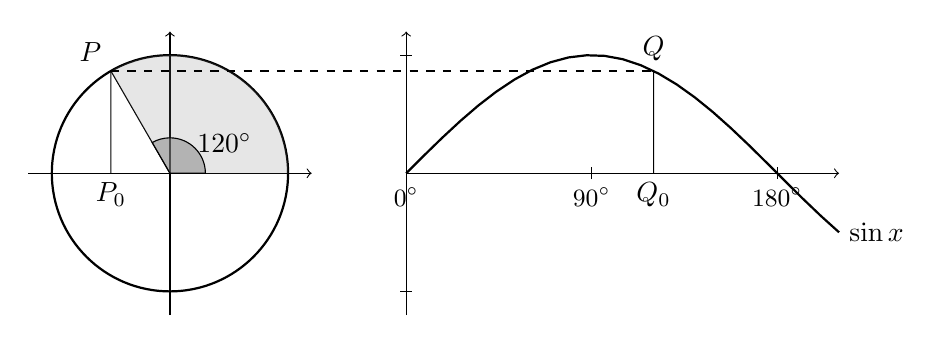
\begin{tikzpicture}[scale=1.5] % 整体放大坐标, 但不影响字号
		\newcommand\iangle{120}
		% 左边的单位圆
		\begin{scope}[xshift=-2cm]
			\draw[->] (-1.2, 0) -- (1.2, 0);
			\draw[->] (0, -1.2) -- (0, 1.2);
			\draw[thick] (0, 0) circle (1);
			\coordinate[label=\iangle: $P$] (P) at (\iangle: 1);
			\coordinate[label=below: $P_0$] (P0) at (P |- 0, 0);
			\draw (0, 0) -- (P);
			\draw (P) -- (P0);
			\fill[fill=gray, fill opacity=0.2]
				(0, 0) -- (0: 1) arc (0: \iangle: 1) -- cycle;
			\filldraw[fill=gray, fill opacity=0.5]
				(0, 0) -- (0: 0.3) arc (0: \iangle: 0.3) -- cycle;
			\node[right] at (\iangle/2: 0.3) {\ang{\iangle}};
		\end{scope}
		% 右边的函数图
		\draw[->] (0, 0) -- ({rad(210)}, 0);
		\draw[->] (0, -1.2) -- (0, 1.2);
		\draw[thick, domain=0: rad(210)] plot (\x, {sin(\x r)})
			node[right] {$\sin x$};
		\foreach \t in {0, 90, 180} {
			\draw ({rad(\t)}, -0.05) -- ({rad(\t)}, 0.05);
			\node[below, outer sep=2pt, font=\small]
				at ({rad(\t)}, 0) {\ang{\t}};
		}
		\foreach \y in {-1, 1} {\draw (-0.05, \y) -- (0.05, \y);}
		\coordinate[label=above: $Q$]
			(Q) at ({rad(\iangle)}, {sin(\iangle)});
		\coordinate[label=below: $Q_0$]
			(Q0) at (Q |- 0, 0);
		\draw (Q) -- (Q0);
		\draw[dashed] (P) -- (Q);
	\end{tikzpicture}
	\caption{正弦函数与单位圆(\textsf{TikZ}实现)}
\end{figure}
\end{document}
